\chapter{Special Topics}

%
%  SECTION 6.1 - Navier-Stokes
%

\section{Deriving the Navier-Stokes Equation}
\label{sec_ns_deriv}

As we'll see, the Navier-Stokes equation follows directly from Newton's second law; however, because it depends on the \emph{deformation} of fluid elements, we need a whole new framework to describe the forces at work. 

\subsection{The Stress Tensor and Vector}

To start, let's consider a fluid element -- I'll draw it as a cube for simplicity but it can be any shape (Figure \ref{fig_deform}).  If we apply a force that's normal to a surface, we'd expect the fluid element to deform by stretching and thinning.  On the other hand, if the \emph{same} force, in the same direction, is applied to a surface that's parallel to it, the deformation will be very different -- the force in this case is called a ``shear force.''  Evidently, the deformation of a fluid element depends not only on the force direction but also on the \emph{surface} direction. 

\begin{figure}
\centering
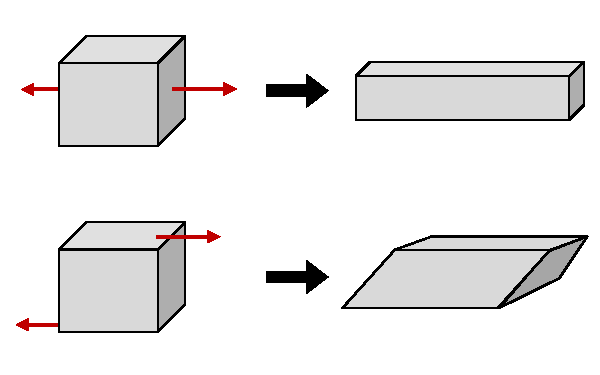
\includegraphics[width=0.9\linewidth]{Figures/Chapter2/fig_deform}
\caption{The deformation of a fluid element depends on both the force direction \emph{and} the direction of the surface. }
\label{fig_deform}
\end{figure}

This, unfortunately, adds a complication to how we must describe the forces that deform a fluid element.  There are three orthogonal directions that the force itself could have, and three orthogonal directions that surface it's applied to could have -- that means we need nine different numbers to fully specify things.  Figure \ref{fig_stress_tensor} shows this graphically; the nine elements together are called the \emph{stress tensor} and are labelled $T_{ij}$, where $i$ specifies the direction of the force, and $j$ the direction of the surface.  The elements of the stress tensor are forces per unit area; for example, the element $T_{xy}$ gives the stress, or force per unit area, acting in the $\unit{x}$ direction on a surface with normal in the $\unit{y}$ direciton.

\begin{figure}
\centering
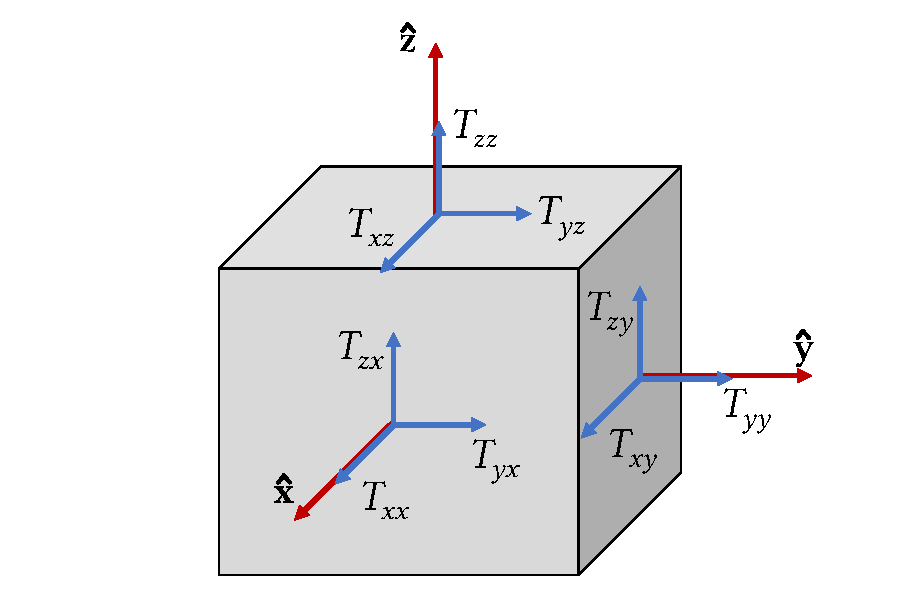
\includegraphics[width=0.7\linewidth]{Figures/Chapter2/fig_stress_tensor}
\caption{The definition of the stress tensor.}
\label{fig_stress_tensor}
\end{figure}

It's common to write the tensors using either ``index notation,'' like $T_{ij}$, or as a matrix:
\[
\tens{T} = \begin{bmatrix}
T_{xx} & T_{xy} & T_{xz} \\
T_{yx} & T_{yy} & T_{yz} \\
T_{zx} & T_{zy} & T_{zz} 
\end{bmatrix}.
\]
Note that the notation for a tensor, $\tens{T}$, is a little different from vectors.  And it turns out that in almost all cases the stress tensor is \emph{symmetric}, so that 
\[
T_{ij} = T_{ji},
\]
which means that we really only have six elements to worry about rather than the full nine.

Suppose we have some surface $S$ with a normal vector $\unit{n}$; the \emph{stress vector} is defined as 
\begin{equation}
\vec{t} = \tens{T} \cdot \unit{n}.
\label{eq_stress}
\end{equation}
Careful here -- that's a dot product between a tensor and a vector, not two vectors, and the result is a vector rather than a scalar.  We can calculate the dot product either by direct summation,
\[
t_i = \sum_{j=1}^3 T_{ij} n_j.
\]
or by matrix multiplicaiton,
\[
\vec{t} = \begin{bmatrix}
T_{xx} & T_{xy} & T_{xz} \\
T_{yx} & T_{yy} & T_{yz} \\
T_{zx} & T_{zy} & T_{zz} 
\end{bmatrix}
\begin{bmatrix}
n_x  \\
n_y  \\
n_z  
\end{bmatrix}.
\]

As a check, let's suppose we have a surface where $\unit{n} = \unit{x}$.  In that case, the stress vector will be
\[
\vec{t} = \begin{bmatrix}
T_{xx} & T_{xy} & T_{xz} \\
T_{yx} & T_{yy} & T_{yz} \\
T_{zx} & T_{zy} & T_{zz} 
\end{bmatrix}
\begin{bmatrix}
1  \\
0  \\
0  
\end{bmatrix} = 
\begin{bmatrix}
T_{xx}  \\
T_{yx}  \\
T_{zx}  
\end{bmatrix},
\]
which makes sense -- the dot product picks out the forces that act on the surface with normal $\unit{x}$.

\subsection{Cauchy's Equation of Motion}

Now we're ready to use Newton's second law to derive a general equation of motion for fluids and other deformable materials.  Consider some ``blob'' of our fluid, with volume $V$ and enclosed by surface $S$; this blob can deform in shape as the fluid moves, but we'll assume our fluid is incompressible, so the total volume can't change.  The force across one small element of area, $dS$, due to the fluid above it, is given by the stress vector $\vec{t}$ multiplied by the area $dS$.  The total force acting on the entire blob due to the surrounding fluid is therefore
\begin{equation}
\vec{F} = \int_S \vec{t} \, dS = \int_S (\tens{T} \cdot \unit{n}) \, dS,
\end{equation}
where I used equation \ref{eq_stress} to write the force in terms of the stress tensor instead of the stress vector.  Now, we can apply the divergence theorem to turn this into an integral over the volume -- even though this is a tensor, it works pretty much the same way:
\[
\vec{F} =  \int_S (\tens{T} \cdot \unit{n}) \, dS = \int_V (\grad \cdot \tens{T} ) \, dV.
\]

So far, we've ignored any forces external to the fluid, but we can add them in now.  I'll stick with gravity; for a small volume of the fluid, the force of gravity will be $\rho dV \vec{g}$, and we can combine this with the stress force above to get
\[
\vec{F} = \int_V (\grad \cdot \tens{T} + \rho \vec{g} ) \, dV.
\]

That's the total force acting on our fluid, and we already know how to write out the acceleration -- that was equation \ref{eq_accel},
\[
\frac{D \vec{u}}{Dt} = \frac{\partial \vec{u}}{\partial t} + (\vec{u} \cdot \vec{\nabla}) \vec{u}.
\]
Newton's second law then gives
\[
\int_V \rho \frac{D \vec{u}}{Dt} \, dV = \int_V (\grad \cdot \tens{T} + \rho \vec{g} ) \, dV.
\]
But this equation holds for \emph{any} volume of any size within our fluid, so the integrands must be equal:
\begin{equation}
\boxed{
\rho \frac{D \vec{u}}{Dt} =\grad \cdot \tens{T} + \rho \vec{g}.
}
\label{eq_cauchy}
\end{equation}
This is called Cauchy's equation of motion.

\subsection{Newtonian Fluids}

So far we've been very general with the stress tensor; specifying different tensors gives us different fluids modelled with Cauchy's equation.  As a first example of a specific stress tensor -- the simplest possible one! -- consider 
\begin{equation}
T_{ij} = -p \, \delta_{ij},
\end{equation}
where $p(x, y, z, t)$ is a scalar function -- it's the \emph{pressure} in the fluid -- and $\delta_{ij}$ is called the Kronecker delta.  If you're not familiar with it, this is a handy function (technically, it's a tensor) that is \emph{one} if the two indices are the same, and \emph{zero} if there's different:
\[
\delta_{ij} = \begin{cases}
0 & i \neq j, \\
1 & i = j \end{cases}.
\]
As a matrix, this stress tensor therefore looks like
\begin{equation}
\tens{T} = \begin{bmatrix}
-p & 0 & 0 \\
0 & -p & 0 \\
0 & 0 & -p
\end{bmatrix}.
\label{eq_stress_ideal}
\end{equation}
This stress tensor defines \emph{ideal fluids}, which are inviscid (no viscosity) and don't include forces of deformation in the stress tensor.  Why the negative sign on the pressure?  Because this is the force of the fluid \emph{outside} the surface pushing on it -- in the opposite direction of the normal vector $\unit{n}$.

Although ideal fluids will make up a large part of our discussion of fluid dynamics, we're here to derive the Navier-Stokes equations, which deal instead with \emph{Newtonian fluids}, which do include the deformation of fluid elements.  To incorporate that, we'll add a term to the ideal fluid stress tensor:
\begin{equation}
T_{ij} = T_{ij}^I + T_{ij}^D,
\end{equation}
where the $I$ indicates the ideal part and the $D$ indicates the part that deals with the deformation.  

Consider, for a moment, a \emph{solid} instead of a fluid.  If the solid is elastic, then pushing on it will cause it to deform in shape, and the stress that results will be proportional to the change in shape.  This makes sense -- it's just like in Hooke's law, where the force of the spring is proportional to the displacement.  A fluid, though, is very different -- pushing on a fluid causes deformation, but the deformation continues even when the force is stopped.  It turns out that for fluids, the stress is proportional to the \emph{velocities} of the change in shape; that is, rather than
\[
t \propto dx,
\]
we have
\[
t \propto du/dx,
\]
for example.  Note a couple of things here:  first, there are three velocities, $u, v, w$, and three directions, $x, y, z$, so we have nine different velocity gradients we can form.  And second, note that these are derivatives with respect to \emph{position}, not time; these are not accelerations.

Now, the most general symmetric tensor that depends \emph{linearly} on these velocity gradients can be written as
\begin{equation}
T_{ij}^D = \mu \left( \frac{\partial u_j}{\partial x_i} + \frac{\partial u_i}{\partial x_j} \right),
\end{equation}
where $\mu$ is the constant of proportionality and is called (of course) the \emph{viscosity}.  Splitting the velocity gradients into two terms likes this ensures the tensor is symmetric.  Although it's cumbersome to do so, and doesn't really gain us anything, I'll write out this tensor in matrix form (you can at least compare with the ideal case in equation \ref{eq_stress_ideal}):
\[
\tens{T}^D = \begin{bmatrix}
2 \mu \partial u / \partial x  &  \mu (\partial v / \partial x + \partial u / \partial y)  &   \mu (\partial w / \partial x + \partial u / \partial z) \\
\mu (\partial u / \partial y + \partial v / \partial x)  & 2\mu  \partial v / \partial y  &  \mu (\partial w / \partial y + \partial v / \partial z) \\
\mu (\partial u / \partial z + \partial w / \partial x)  &  \mu (\partial v / \partial z + \partial w / \partial y) & 2\mu  \partial w / \partial z
\end{bmatrix}.
\label{eq_stress_newtonian}
\]

Adding in the ideal component, the total stress tensor is
\begin{equation}
\boxed{
T_{ij} = -p \delta_{ij} +  \mu \left( \frac{\partial u_j}{\partial x_i} + \frac{\partial u_i}{\partial x_j} \right).
}
\end{equation}
This defines a \emph{Newtonian fluid}.  But you should know that there's plenty of examples of \emph{non-Newtonian fluids,} as well -- paint and blood are two good examples.  Non-Newtonian fluids can be nonlinear in the velocity gradients, and can sometimes depend not just on the current state of the fluid, but on the past state as well -- some of these fluids can have a ``memory.''  These kinds of fluids are well outside the scope of this book, however.

\begin{example}[Plane parallel shear flow]
Recall our example from Section \ref{sec_imp} -- we had an impulsively moved boundary, which put the fluid into plane parallel shear flow given in general by $u(y)$.  For simplicity, we'll suppose the boundary is at $y=0$ and the flow exists above it.  What is the stress on the boundary from the fluid?

For flow of this type, the stress tensor becomes
\begin{equation}
\tens{T} = \begin{bmatrix}
-p & \mu \partial u / \partial y & 0 \\
\mu \partial y / \partial y & -p & 0 \\
0 & 0 & -p
\end{bmatrix},
\end{equation}
and we can calculate the stress vector using equation \ref{eq_stress}, with $\unit{n} = \unit{y}$ for the boundary surface:
\[
\vec{t} = \begin{bmatrix}
-p & \mu \partial u / \partial y & 0 \\
\mu \partial y / \partial y & -p & 0 \\
0 & 0 & -p
\end{bmatrix}
\begin{bmatrix}
0 \\ 1 \\ 0
\end{bmatrix}.
\]
Carrying out the matrix multiplication gives
\[
\vec{t} = \mu \frac{\partial u}{\partial y} \unit{x} - p \unit{y}.
\]
This result makes sense: there's a viscous force along the boundary caused by friction with the fluid, and a force pushing downward on the surface from the fluid above.
\end{example}

We're finally ready to derive the Navier-Stokes equation, which is just Cauchy's equation of motion with the stress tensor for Newtonian fluids.  I'm going to write out the calculation in index notation, which is a little easier to deal with, starting with Cauchy's equation,
\[
\rho \frac{Du_i}{Dt} = \sum_{j=1}^3 \frac{\partial T_{ij}}{\partial x_j} + \rho g_i
\]
(compare with the vector version in equation \ref{eq_cauchy}).  We only tricky thing here is the divergence of the stress tensor,
\[
\sum_{j=1}^3 \frac{\partial T_{ij}}{\partial x_j} = \sum_{j=1}^3 \frac{\partial }{\partial x_j} \left[ -p \delta_{ij} + \mu \left( \frac{\partial u_j}{\partial x_i} + \frac{\partial u_i}{\partial x_j} \right) \right],
\]
which is three derivatives.  We'll tackle each separately.

First is the pressure term,
\[
\sum_{j=1}^3 \frac{\partial }{\partial x_j} \left( -p \delta_{ij} \right) = - \sum_{j=1}^3  \frac{\partial p}{\partial x_j} \delta_{ij} = -\frac{\partial p}{\partial x_i}.
\]
Notice that the Kronecker delta \emph{collapsed} the sum -- every term was zero except for the one where $j = i$.  

The next derivative is
\[
\sum_{j=1}^3 \frac{\partial }{\partial x_j} \left( \mu \frac{\partial u_j}{\partial x_i} \right) = \mu \frac{\partial }{\partial x_i} \sum_{j=1}^3 \frac{\partial u_j}{\partial x_j},
\]
where I took the derivative with respect to $x_i$ outside the sum (which is over $j$).  Now, the term in the sum is familiar, even if it's hidden a bit -- it's the divergence of the fluid velocity:
\[
\sum_{j=1}^3 \frac{\partial u_j}{\partial x_j} = \frac{\partial u}{\partial x} + \frac{\partial v}{\partial y} + \frac{\partial w}{\partial z} = \grad \cdot \vec{u}.
\]
But we're assuming an incompressible flow, so the divergence is \emph{zero}, and this derivative goes away.

Finally, we have the third derivative,
\[
\sum_{j=1}^3 \frac{\partial }{\partial x_j} \left( \mu \frac{\partial u_i}{\partial x_j} \right) = \mu \sum_{j=1}^3 \frac{\partial^2 u_i}{\partial x_j^2},
\]
and putting all three together gives us 
\[
\rho \frac{Du_i}{Dt} = -\frac{\partial p}{\partial x_i} + \mu \sum_{j=1}^3 \frac{\partial^2 u_i}{\partial x_j^2} + \rho g_i.
\]
Dividing both sides by the density $\rho$ (and remembering that the kinematic viscosity is $\nu = \mu / \rho$) and using vector notation gives us, at long last, the Navier-Stokes equation,
\begin{equation}
\boxed{
\frac{D \vec{u}}{Dt} = - \frac{1}{\rho} \grad p + \nu \nabla^2 \vec{u} + \vec{g}.
}
\end{equation}


%
% --- SECTION - ADVANCED TOPIC 2 ---
% 

\section{Boundary Layers}
\label{sec_boundary_layers}

The presence of a boundary layer in a fluid is one of the big differences between viscous flow and inviscid.  To explore boundary layers further, let's set up a fairly simple situation.  Consider fluid in the region $y \ge 0$, above a rigid boundary along $y=0$.  Suppose the flow is given by
\begin{equation}
\vec{u} = [\alpha x, -\alpha y, 0],
\end{equation}
where $\alpha$ is some constant.  We've seen this type of flow before, in Chapter 1 -- it's the flow about a stagnation point.  The streamlines are shown in Figure \ref{fig_boundary_stream}.

\begin{figure}
\centering
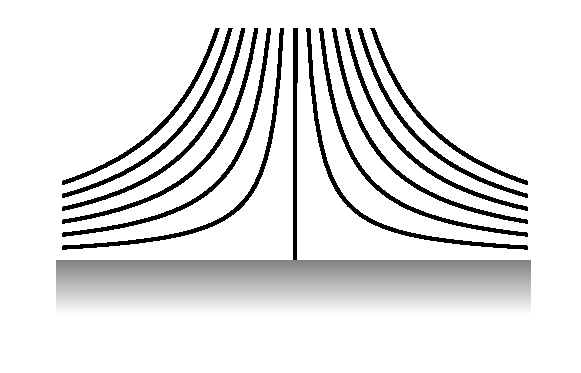
\includegraphics[width=0.6\linewidth]{Figures/Chapter2/fig_boundary_stream}
\caption{Streamlines for flow about a stagnation point.  The fluid lies above the $x$-axis.}
\label{fig_boundary_stream}
\end{figure}


Now, this flow satisfies the Navier-Stokes equation, with a pressure given by
\begin{equation}
\label{eq_boundary_pressure}
p(x, y) = -\frac{1}{2} \rho \alpha^2 ( x^2 + y^2) + \text{ constant}.
\end{equation}
However, it \emph{doesn't} satisfy the no-slip boundary condition -- the fluid velocity isn't zero at the boundary!  This is actually fine if we're dealing with an inviscid fluid, where we expect the flow to be directed along the boundary, but doesn't work for a viscous fluid.  It also has no indications of a boundary layer.

We need to fix things up, then, to account for the boundary layer and viscosity.  We can do that by changing our flow slightly to
\begin{equation}
\label{eq_boundary_trial}
\vec{u} = [\alpha x f'(\eta), -\sqrt{\nu \alpha} f(\eta), 0],
\end{equation}
where
\[
\eta = \sqrt{ \frac{\alpha}{\nu}} y
\]
is a dimensionless length parameter.  Here, the function $f(\eta)$ is an unknown function that we'll solve for shortly; notice that if $f(\eta) = \eta$, we get back our original flow about a stagnation point.  However, in order to satisfy the no-slip condition and get zero velocity at $y=0$, we need $f \to 0$ \emph{and} $f' \to 0$ when $\eta \to 0$.  Clearly $f(\eta) = \eta$ won't do the trick.  On the other hand, we do expect the flow far away from the boundary to look like our original stagnation point flow; we'll return to this later.

To find the function $f(\eta)$ properly, then, we need to make sure that this flow still satisfies the Navier-Stokes equation.  If we plug in the velocity in Equation (\ref{eq_boundary_trial}) into the Navier-Stokes equation, the $x$ and $z$ equations become
\begin{equation}
\label{eq_boundary_ns1}
\alpha^2 x f'^2 - \alpha^2 x f f'' = -\frac{1}{\rho} \frac{\partial p}{\partial x} + \alpha^2 x f'''
\end{equation}
and
\begin{equation}
\sqrt{\alpha^3 \nu } ff' = \frac{1}{\rho} \frac{\partial p}{\partial y} - \sqrt{\alpha^3 \nu} f'',
\end{equation}
respectively.  Let's rearrange the second equation slightly to get
\[
-\frac{1}{\sqrt{\alpha^3 \nu}} \frac{1}{\rho} \frac{\partial p}{\partial y} = \frac{1}{2} \frac{d}{d\eta} f^2 + \frac{d}{d\eta} f'.
\]
We can then replace the $\partial y$ derivative with $\partial \eta$, since
\[
\frac{d\eta}{dy} = \sqrt{\frac{\alpha}{\nu}},
\]
to get
\[
-\frac{1}{\alpha \nu \rho} \frac{\partial p}{\partial \eta} = \frac{1}{2} \frac{d}{d\eta} f^2 + \frac{d}{d\eta} f'.
\]
Finally, integrate with respect to $\eta$:
\[
-\frac{1}{\alpha \nu \rho} p = \frac{1}{2} f^2 + f' + g(x),
\]
where $g(x)$ is the integration ``constant.''  This is a useful result:  if we now take the derivative with respect to $x$, we can see that 
\[
\frac{\partial p}{\partial x} \propto \frac{\partial g}{\partial x}.
\]
In other words, $\partial p / \partial x$ is at best a function of $x$.

We can now return to the other Navier-Stokes equation, Equation (\ref{eq_boundary_ns1}), and separate variables so that all $x$ terms are on one side and all $\eta$ terms are on the other:
\[
-\frac{1}{\alpha^2 \rho x} \frac{\partial p}{\partial x} = f'^2 - ff'' - f'''.
\]
Since $x$ and $\eta$ (which is really just $y$) are independent, each side of this equation must be a constant.  What is the value of that constant?  To find it, we'll compare with the inviscid solution for the pressure, Equation (\ref{eq_boundary_pressure}).  To have our pressures agree, we need the constant to be one.

Finally, then, we have our last equation we need to solve,
\begin{equation}
f''' + ff'' - f'^2 + 1 = 0.
\end{equation}
As we've discussed above, the boundary conditions are
\[
f(0) = 0; \quad f'(0) = 0; \quad \text{and} \quad f'(\infty) = 1,
\]
where the last condition ensures that we return to our original flow (with $f(\eta) = \eta$) far away from the boundary.

This equation must be solved numerically, but it can be tricky to do so while making sure the boundary conditions match; the results are shown in Figures \ref{fig_boundary_result1} and \ref{fig_boundary_result2}.  As you can see, there is now a small boundary layer where the velocity drops to zero, but away from the boundary the flow is indistinguishable from the inviscid case.  Despite the complexity of this example, it's a good one for exploring exactly how the boundary layer develops for viscous flows.

\begin{figure}
\centering
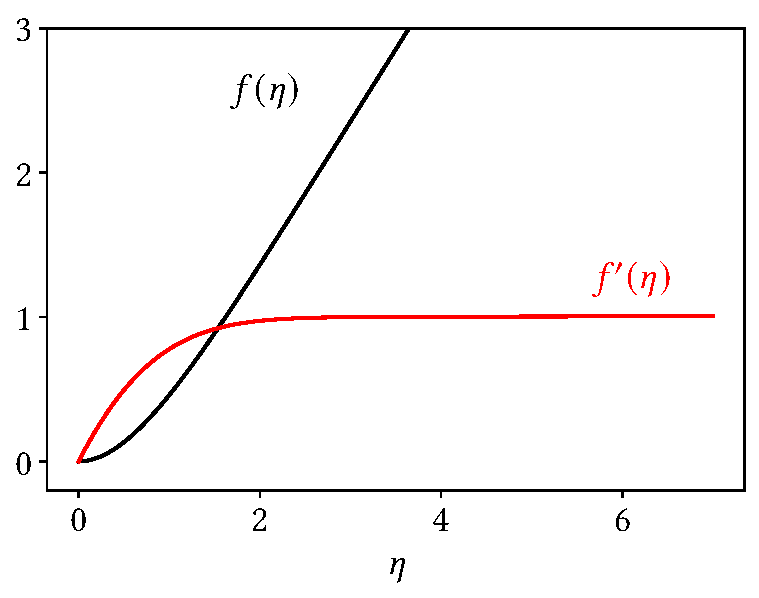
\includegraphics[width=0.7\linewidth]{Figures/Chapter6/fig_boundary_result1}
\caption{The function $f(\eta)$ (black) and $f'(\eta)$ (red).  Note that the boundary layer is clear -- it extends out to around $\eta \sim 2$.  After that, $f(\eta) \approx \eta$. }
\label{fig_boundary_result1}
\end{figure}

\begin{figure}
\centering
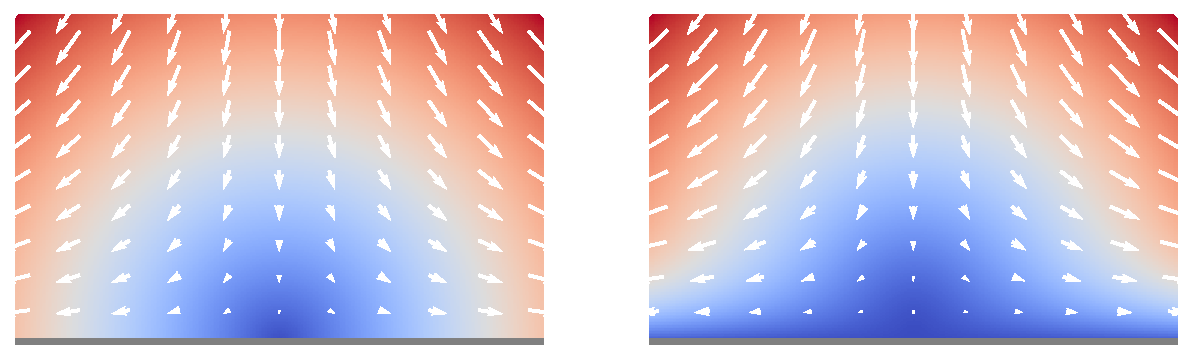
\includegraphics[width=\linewidth]{Figures/Chapter6/fig_boundary_result2}
\caption{Vector plots of the invisid flow (left) and viscous flow (right).  The boundary layer can be clearly seen in the flow -- the blue colour indicates small velocity. }
\label{fig_boundary_result2}
\end{figure}

%
% --- SECTION - ADVANCED TOPIC 3 ---
% 

\section{The Dam Break Problem}

Coming soon.


%
% --- SECTION - ADVANCED TOPIC 4 ---
% 


\section{Spherical Flows}

Coming soon.

%
% --- SECTION - ADVANCED TOPIC 5 ---
% 

\section{Stellar Structure}

In this section we turn our attention to using fluid dynamics to explore the structure of \emph{stars}.  There are two pretty big things which we'll to include in addition to the usual theory:  the presence of \emph{self-gravity}, meaning that the star is massive enough that we have to take its own gravity into account, and the presence of energy generation and transport -- stars create energy through nuclear fusion at their core and transport it to the surface via mechanisms like radiative transport and convection.

\subsection{Newtonian Gravity}

We've already discussed, way back in Chapter 3, using a \emph{gravitational potential} to describe gravity, and we'll continue that here.  If $\vec{g}$ is the gravitation field as usual, then we can write it in terms of a gradient of a scalar,
\begin{equation}
\vec{g} = -\grad \Phi.
\end{equation}
It'll be much easier to work with the gravitational potential rather than the field.  

One difference from what we've done before, however, is the form that the field $\vec{g}$ takes; after all, we're not on the surface of the Earth anymore, where $\vec{g} = [0, 0, -g]$, for example.  Instead, it's due to the entire star itself, and we have to add up all the contributions from each bit of it.  From Newton's law of gravity, the force on a mass $m$ due to a mass $m'$ is 
\[
\vec{F}(\vec{r}) = -\frac{G m m'}{|\vec{r} - \vec{r}'|^3} (\vec{r} - \vec{r}'),
\]
where $\vec{r}$ is the location of mass $m$ and $\vec{r}'$ is the location of mass $m'$.  From Newton's second law, the mass feels an acceleration
\[
\vec{g}(\vec{r}) = \frac{\vec{F}(\vec{r})}{m} = -\frac{G m'}{|\vec{r} - \vec{r}'|^3} (\vec{r} - \vec{r}')
\]
(and $\vec{g}$ is often called the gravitational field).  At this point it's simple to generalize to get the field due to a continuous mass distribution like a star:
\begin{equation}
\vec{g}(\vec{r}) = -G \int_V \frac{ \rho(\vec{r}') (\vec{r} - \vec{r}')}{|\vec{r} - \vec{r}'|^3} \, d\tau'.
\end{equation}

This is the connection between the mass density $\rho(\vec{r})$ and the field $\vec{g}(\vec{r})$; what about the potential $\Phi(\vec{r})$?  We find the potential via Poisson's equation,
\begin{equation}
\label{eq_poisson}
\boxed{
\nabla^2 \Phi(\vec{r}) = 4 \pi G \rho(\vec{r}).
}
\end{equation}
This is the main equation of Newtonian gravity.


\subsection{Energy Transport}

A star generates energy at its core through fusion; stars on the so-called main sequence burn hydrogen to helium.  This process is of course quite complicated, requiring understanding of the various nuclear processes that happen, but if we ignore the details, suppose that $\epsilon$ is the total energy released through fusion per unit mass per unit time -- that means
\[
\int_V \epsilon \rho \, d\tau
\]
is the \emph{rate} at which energy is generated within the star.

The star then transports that energy to the surface.  There are two main processes that accomplish this:  radiative transport, in which energy is carried by photons, and adiabatic convection, in which energy is carried by matter.  Again, ignoring the details for now, we'll call $\vec{F}$ the \emph{flux} of energy, and the quantity
\[
\int_S \vec{F} \cdot d\vec{a}
\]
represents the rate that energy is transported through a surface $S$ with area vector $d\vec{a}$.

In addition to these two processes, the energy within a star can change due to the work done by the pressure in the fluid and the work done by gravity.  If we add up all the contributions, the total rate of energy change is
\begin{equation}
\label{eq_energy_all}
\frac{dE}{dt} = - \int_S p \vec{u} \cdot d\vec{a} + \int_V \vec{g} \cdot \vec{u} \rho d\tau + \int_V \epsilon \rho d\tau - \int_S \vec{F} \cdot d\vec{a}
\end{equation}
(note the negative sign on the pressure and flux terms to account for the fact that the area vector $d\vec{a}$ points outward).

The total energy $E$ can be written as the sum of the kinetic energy $T$ and the internal thermal energy (per unit mass) $U$, so the change in energy is
\[
\frac{dE}{dt} = \frac{d}{dt}\int_V \left( \frac{1}{2} \vec{u}^2 + U \right) \rho d\tau.
\]
If we move the derivative inside the integral, it becomes the material derivative, 
\[
\frac{dE}{dt} = \int_V \left[ \frac{D}{Dt}\left( \frac{1}{2} \vec{u}^2 \right) + \frac{DU}{Dt} \right] \rho d\tau.
\]
We can then use the divergence theorem to turn the surface integrals in equation (\ref{eq_energy_all}) into volume integrals, and, since the volume is arbitrary, drop the integrals to get
\begin{equation}
\label{eq_energy_all2}
\rho \left[ \frac{D}{Dt}\left( \frac{1}{2} \vec{u}^2 \right) + \frac{DU}{Dt} \right] = -\grad \cdot (p\vec{u}) + \rho \vec{g} \cdot \vec{u} + \rho \epsilon - \grad \cdot \vec{F}.
\end{equation}

One last thing:  we can use Euler's equation (assuming the star is made of an ideal fluid, a good assumption) to get rid of the kinetic energy term, and the continuity equation to clean things up a bit more.  Problem \ref{prob_energy_change} has the details; equation (\ref{eq_energy_all2}) becomes
\begin{equation}
\label{eq_thermal_energy}
\boxed{
\frac{DU}{Dt} = \frac{p}{\rho^2} \frac{D\rho}{Dt} + \epsilon - \frac{1}{\rho} \grad \cdot \vec{F}.
}
\end{equation}
This equation says that the internal thermal energy of a fluid element can change in three different ways:  by a change in density, by generating energy via fusion, or by transporting energy away. 

\subsection{Equations of Stellar Structure}

Equations (\ref{eq_poisson}) and (\ref{eq_thermal_energy}), along with Euler's equation and the continuity equation, constitute the theory of stellar structure.  For convenience, I'll put them all together:
\begin{align*}
\frac{D \uu}{Dt} = -\frac{1}{\rho} \grad p + \vec{g} & \quad \text{(Euler's equation),} \\
\frac{\partial \rho}{\partial t} + \vec{\nabla} \cdot (\rho \vec{u} ) = 0 & \quad \text{(continuity equation),} \\
\nabla^2 \Phi = 4 \pi G \rho & \quad \text{(self-gravity),} \\
\frac{DU}{Dt} = \frac{p}{\rho^2} \frac{D\rho}{Dt} + \epsilon - \frac{1}{\rho}  \grad \cdot \vec{F} & \quad \text{(thermal enegry).}
\end{align*}

Now, that's four equations, but if you count the unknowns, they're actually five:  the velocity $\vec{u}$, the pressure $p$, the density $\rho$, the gravitational potential $\Phi$ (or the field $\vec{g}$), and the thermal energy $U$.  Note that $\epsilon$, the rate of energy generation, and $\vec{F}$, the flux of energy, aren't strictly unknowns here; they require additional theory to compute, depending on what exactly we're modelling, so think of them as \emph{inputs} into the theory of stellar structure. But what's the fifth equation?  As discussed back in Section \ref{sec_comp_fluids}, we need an \emph{equation of state}.  More on what we'll use in a bit.

These equations are extremely complicated to solve, even numerically.  But we can make some headway and produce simple but useful models of stars and other objects with a few assumptions:
\begin{itemize}
\item That the fluid has no time dependence -- it's \emph{steady flow}.  But we'll also assume no time dependence for every variable, including energy $U$.
\item Even stronger, we'll assume the fluid is \emph{static} -- that $\vec{u} = 0$.  Our stars will be made up of a fluid that doesn't actually flow.
\item And we'll assume spherical symmetry -- there's only a dependence on the distance from the origin, $r$.
\end{itemize}

As you might guess, these assumptions drastically simplify our equations; they become
\begin{align}
\frac{dp}{dr} = -\rho \frac{d\Phi}{dr}  & \quad \text{(Euler's equation),} \label{eq_star_1} \\
0 = 0 & \quad \text{(continuity equation),} \\
\frac{1}{r^2} \frac{d}{dr} \left(r^2 \frac{d\Phi}{dr} \right) = 4 \pi G \rho & \quad \text{(self-gravity),} \label{eq_star_3} \\
\epsilon = \frac{1}{\rho} \frac{1}{r^2} \frac{d}{dr} ( r^2 F) & \quad \text{(thermal enegry).} \label{eq_star_4}
\end{align}
But even better, we can combine the first and third equation in the following way.  First, integrate the third equation for self-gravity, so that
\[
r^2 \frac{d\Phi}{dr} = \int_0^r 4\pi G \rho(r') r'^2 \, dr'.
\]
But the right hand side is (almost) just the mass contained inside a radius $r$:
\[
M(r) = 4\pi \int_0^r \rho(r') r'^2 \, dr',
\]
so the third equation can be written
\begin{equation}
\frac{d\Phi}{dr} = \frac{GM(r)}{r^2},
\end{equation}
and substituted into the first equation, giving
\begin{equation}
\label{eq_star_1b}
\boxed{
\frac{dp}{dr} = - \frac{GM(r) \rho}{r^2}.
}
\end{equation}
This is the equation for \emph{hydrostatic equilibrium}: the inward force of gravity is balanced by the outward pressure of the fluid, allowing the star to be static.

The fourth equation, for thermal energy, says that any energy produced ($\epsilon$) within the star must be balanced by the energy flux ($F$) -- this is a statement of \emph{thermal equilibrium}.  It's more common to write this in terms of the \emph{luminosity} $L$, which is the energy emitted per unit time by a radial shell of the fluid, in which case the flux is
\begin{equation}
F = \frac{L}{4\pi r^2}.
\end{equation}
Then the fourth equation becomes, in terms of the luminosity,
\begin{equation}
\boxed{
\frac{dL}{dr} = 4\pi r^2 \rho \epsilon.
}
\end{equation}

Finally, we need to discuss the equation of state -- but there are two possibilities.  If we assume the pressure in the fluid is provided purely by the radiation emitted by the gas, then the equation of state is
\begin{equation}
p_\text{rad} = \frac{1}{3} aT^4,
\end{equation}
where $a = 7.566 \times 10^{-16}$ J m$^{-3}$ K$^{-4}$ is called the radiation constant (it's related to the Stefan-Boltzmann constant if you're more familiar with that).  There could also be a contribution to the pressure from the fluid itself.  If we assume it's an ideal gas, then we have the usual (see Section \ref{sec_comp_fluids}) gas law
\begin{equation}
p_\text{gas} = \rho \kappa T.
\end{equation}

In general, both of these sources of pressure are important, and we should include them both:
\begin{equation}
p = p_\text{rad} + p_\text{gas} = \frac{1}{3} aT^4 + \rho \kappa T.
\end{equation}
Suppose that the gas pressure makes up some fraction of the total -- call the fraction $\beta$, so that
\[
p_\text{gas} = \beta p = \rho \kappa T.
\]
Radiation pressure makes up the rest:
\[
p_\text{rad} = (1 - \beta) p = \frac{1}{3} aT^4.
\]
We can use these two equations to eliminate the temperature, giving the pressure in terms of the density alone.  It turns out to take on the simple form
\begin{equation}
\label{eq_eos_edd}
p = k \rho^{4/3},
\end{equation}
where the constant $k$ is given by
\[
k = \left[ \frac{3 (1-\beta) \kappa^4}{a \beta^4} \right]^{1/3}.
\]
Stars with an equation of state given by equation (\ref{eq_eos_edd}) are called \emph{Eddington standard models}.  But it turns out that the general form of the equation of state, that $p \propto \rho^\gamma$, arises in many situations -- we've seen one already in Section \ref{sec_comp_fluids} with adiabatic processes, where $\gamma$ is related to the ratio of specific heats.  Models which have this form are called \emph{polytropes} and deserve a bit more discussion.

\subsection{Polytropic Models}

Suppose, then, we take as our equation of state the general form
\begin{equation}
\label{eq_polytrope}
p = k \rho^\gamma.
\end{equation}
What does this do for us?  We can use it to eliminate either pressure or density from equation (\ref{eq_star_1b}).  First rearrange and take the derivative of equation (\ref{eq_star_1b}) to get
\[
\frac{d}{dr} \left( \frac{r^2}{\rho} \frac{dp}{dr} \right) = -G \frac{dM}{dr},
\]
and then use $dM/dr = 4\pi r^2 \rho$ to get
\[
\frac{d}{dr} \left( \frac{r^2}{\rho} \frac{dp}{dr} \right) = - 4 \pi G \rho.
\]
Now we can replace the pressure using equation (\ref{eq_polytrope}); the derivative of it is
\[
\frac{dp}{dr} = k \gamma \rho^{\gamma - 1} \frac{d\rho}{dr}.
\]
Plugging this into the equation above gives us an expression involving only the density:
\begin{equation}
\label{eq_star_density}
\frac{k\gamma}{r^2} \frac{d}{dr} \left( r^2 \rho^{\gamma - 2} \frac{d\rho}{dr} \right) = -4\pi G \rho.
\end{equation}

We could in principle solve this differential equation for the density $\rho(r)$, but this is not a very simple-looking equation.  We can clean it up a bit by introducing two dimensionless parameters.  The first is a scaled density parameter, $\varrho$, such that
\begin{equation}
\label{eq_varrho}
\rho(r) = \rho_c \varrho^n(r),
\end{equation}
where $\rho_c$ is a constant (with units of density) and the index $n$ is related to the parameter $\gamma$ by
\begin{equation}
\gamma = \frac{n+1}{n}.
\end{equation}
The second parameter is a scaled radius; define 
\begin{equation}
\eta = \frac{r}{\lambda},
\end{equation}
where $\lambda$ is a constant dependent on the index $n$:
\begin{equation}
\lambda^2 = \frac{(n+1) k \rho_c^{(1-n)/n}}{4\pi G}.
\end{equation}
In terms of these two new variables, equation (\ref{eq_star_density}) becomes
\begin{equation}
\boxed{
\frac{1}{\eta^2} \frac{d}{d\eta} \left( \eta^2 \frac{d\varrho}{d\eta} \right) = - \varrho^n.
}
\end{equation}
This is called the \emph{Lane-Emden equation}, and the solutions to it are polytropic models of stars.

We'll solve the Lane-Emden equation in a moment, but first we need to discuss the boundary conditions.  The first is pretty simple: we want the density at the centre of the star to be \emph{finite}, so we'll choose
\begin{equation}
\varrho(0) = 1.
\end{equation}
This makes the constant $\rho_c$ the value of the density at the centre of the star (hence the subscript $c$), something that can be fit to model a particular system.  The second boundary condition needs a bit more motivation.  

Consider a small volume at the centre of the star with radius $\delta$.  The volume within $\delta$ is
\[
V = \frac{4}{3} \pi \delta^3,
\]
and the mass enclosed by that radius is
\[
M = \frac{4\pi}{3} \bar{\rho} \delta^3,
\]
where $\bar{\rho}$ is the \emph{average} density within the volume.  From equation (\ref{eq_star_1b}), the change in pressure is then
\[
\frac{dp}{dr} = -\frac{4\pi}{3} G \bar{\rho}^2 \delta.
\]
In the limit as $\delta \to 0$, then, we have that
\[
\frac{dp}{dr} \to 0.
\]
Now, for a polytropic model, the density is proportional to the pressure, so this also says
\[
\frac{d\rho}{dr} \to 0 \quad \text{as} \quad r \to 0.
\]
In terms of the dimensionless variables, our second boundary condition becomes
\begin{equation}
\frac{d\varrho}{d\eta} = 0 \quad \text{at} \quad \eta = 0.
\end{equation}

We're ready to solve the Lane-Emden equation and produce our first models for a star.  It turns out, however, that there's only a few cases for which it can be solved analytically:  for values of $n = 0, 1, 5,$ and $n = \infty$.  I'll walk you through a couple here, and you can work on Problem \ref{prob_lane_emden} for others.

\begin{example}[n = 0]
The easiest case is $n = 0$, in which case the Lane-Emden equation becomes
\[
\frac{1}{\eta^2} \frac{d}{d\eta} \left( \eta^2 \frac{d\varrho}{d\eta} \right) = -1.
\]
This case be solved by integrating twice, giving
\[
\varrho(\eta) = c_1 - \frac{c_2}{\eta} - \frac{1}{6} \eta^2.
\]
Fitting the boundary conditions requires $c_1 = 1$ and $c_2 = 0$, and the dimensionless density is
\[
\varrho(\eta) = 1 - \frac{1}{6} \eta^2.
\]
Notice that the density drops to zero at a radius $\eta_s = \sqrt{6}$ -- this is the surface of the star.  

But this is a strange model for star, since, according to equation (\ref{eq_varrho}), the density is actually constant $\rho_c$ throughout.  So, not a very good model of a star -- but it does turn out to be a reasonable model of a rocky planet like the Earth.
\end{example}

\begin{example}[n = 5]
If $n = 5$, the Lane-Emden equation becomes
\[
\frac{1}{\eta^2} \frac{d}{d\eta} \left( \eta^2 \frac{d\varrho}{d\eta} \right) = -\varrho^5.
\]
This has the solution
\[
\varrho(\eta) = \frac{1}{\sqrt{1 + \eta^2/3}}.
\]
Unlike the previous example, where the density dropped to zero at a certain point, in this case the density becomes zero at infinity -- evidently $n=5$ models an infinitely large star!  Actually, this case -- usually called a \emph{Plummer sphere} -- can be a simple model of systems of stars like globular clusters or galaxies.
\end{example}

Neither of these two examples were particularly good model for \emph{stars}, the objects we set out to investigate in the first place.  Other values of $n$ do a better job of that:  $n = 1.5$ provides a good model of convective star cores as well as low mass white dwarfs, for example, and $n = 3$, which correspond to the Eddington standard model, models the radiation zones of main-sequence stars as well as high mass white dwarfs.  However, those cases don't have an analytic solution and the Lane-Emden equation must be solved numerically.  The densities of some of these models are shown in Figure \ref{fig_polytropes}.

\begin{figure}
\centering
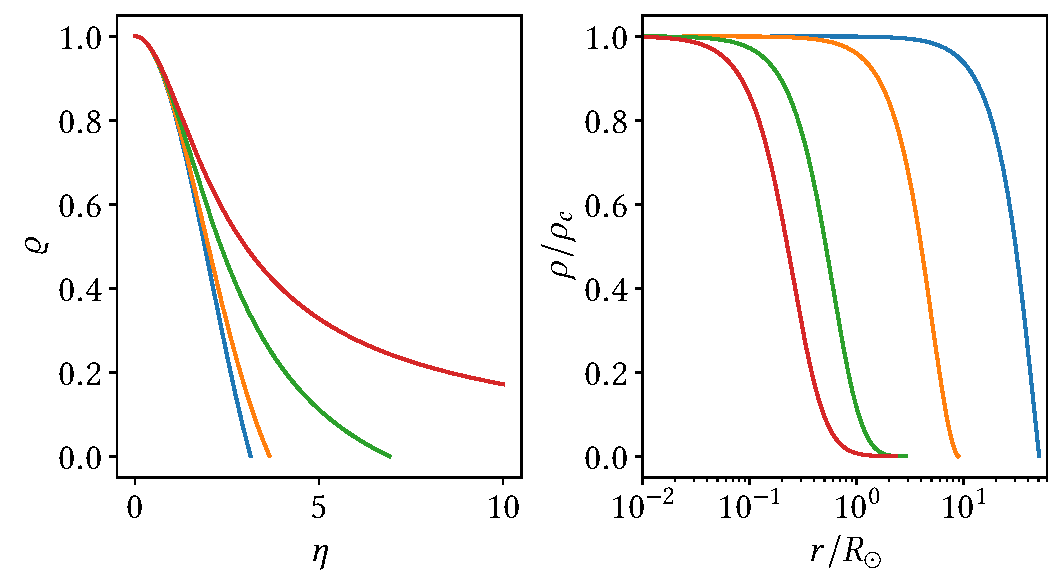
\includegraphics[width=0.9\linewidth]{Figures/Chapter6/fig_polytropes}
\caption{Density profiles for various polytropes.  Left: the dimensionless density parameter $\varrho(\eta)$.  Right: the density $\rho(r)$, using solar values for various constants, plotted in terms of the central density of the sun and solar radii.  Blue: $n = 1$.  Orange: $n = 1.5$. Green: $n=3$.  Red: $n=5$. }
\label{fig_polytropes}
\end{figure}


%
% --- SECTION - ADVANCED TOPIC 6 ---
% 

\section{Numerical Methods}

Or stellar atmospheres?



\section*{Problems}
\addcontentsline{toc}{section}{Problems}
\markright{Problems}%

\begin{problem}[Pressure and the Stress Tensor]
\label{prob_pressure} 
Show that, for the Newtonian stress tensor (equation \ref{eq_stress_newtonian}), the pressure is the negative of the average of the three normal stresses.  Explain why this makes sense.
\end{problem}

\begin{problem}[Rate of change of thermal energy]
\label{prob_energy_change} 

(a) From Euler's equation (\ref{eq_euler}), derive the \emph{mechanical energy equation},
\[
\frac{D}{Dt} \left( \frac{1}{2} \vec{u}^2 \right) = -\frac{1}{\rho} \vec{u} \cdot \grad p + \vec{u} \cdot \vec{g}.
\]
(\emph{Hint}: Start by taking the dot product of Euler's equation with $\vec{u}$.)

(b) From the continuity equation (\ref{eq_continuity}), show that you can write the divergence of the velocity as
\[
\grad \cdot \vec{u} = -\frac{1}{\rho} \frac{D\rho}{Dt}.
\]

(c) Thus, show that equation (\ref{eq_energy_all2}) becomes equation (\ref{eq_thermal_energy}).

\end{problem}


\begin{problem}[Polytrope with $n=1$]
\label{prob_lane_emden} 
Consider a polytrope with $n=1$.  

(a) Solve the Lane-Emden equation to find the dimensionless density $\varrho(\eta)$ and calculate the value of the surface $\eta_s$.

(b) Show that the total mass within the star is $M = 4\pi^2 \rho_c \lambda^3$.

(c) Define the dimensionless pressure as 
\[
\mathscr{p} = \frac{p}{k\rho_c^n}
\]
and find $\mathscr{p}(\eta)$ for this case.

(d) Plot the dimensionless density and dimensionless pressure.
\end{problem}




